\chapter{Trabalhos relacionados} \label{cap:literatura}
  
Este capítulo descreve os principais trabalhos relacionados encontrados na literatura referenciada neste trabalho. A primeira seção cita a primeira referência literária encontrada na execução deste trabalho que realiza comparações de métodos de previsão de demanda. A segunda seção cita pesquisas relacionadas ao tema deste trabalho, a predição de demanda em restaurantes universitários, contendo estudos relacionados com uma parte dos métodos executados neste trabalho que são os modelos de redes neurais MLP, e o diferencial deste trabalho em relação aos outros é a inclusão de redes neurais recorrentes modernas, denominadas GRU, fundamentadas no tópico \ref{sec:GRU}. A última seção cita o maior volume de referências encontradas durantes as pesquisas de predição de demanda em geral, e que não corresponderam ao tema deste trabalho.

    \section{Trabalho de comparações de métodos de previsão de demanda.}
       \citeonline{Junior2007} Realiza um trabalho de comparação entre os métodos estocásticos (Método de suavização exponencial, modelos de Box-Jenkins) e modelos de aprendizado de máquina (Redes Neurais), ilustrados na Figuras \ref{fig: metodosPrevisaoDemanda}, os quais são usados para a previsão da demanda de produtos cosméticos distribuídos em séries temporais. Entre as Redes Neurais, encontramos redes do tipo \textit{feedforward} com o algoritmo de treino por \textit{backpropagation} que foi o principal foco no trabalho de previsão do R.U na Universidade Federal de Viçosa e na Universidade Estadual Paulista Júlio de Mesquita Filho, e que também fundamentou parte do desenvolvimento deste trabalho de predição no ICT Unifesp. Neste trabalho do autor, também são analisadas diversas medidas de performance preditivas e é feito uma análise comparativa final destas medidas entre os métodos citados.
    
    \section{Previsão de demanda em restaurantes universitários}
        No estudo estatístico feito por \citeonline{Landim2016}, foi analisada a correlação entre a temperatura e o consumo de refeições nos dias de vendas do restaurante universitário do campus ICT-Unifesp, sendo que os dados continham apenas uma pequena amostra das vendas do segundo semestre de 2016. Devido ao baixo volume de ocorrências, os dados foram submetidos à reamostragem via bootstrap. De acordo com os gráficos das amostras, identificou-se que a correlação mostrada nos gráficos da primeira metade do semestre e do período total do semestre formaram distribuições bimodais. Porém, na segunda metade do semestre formou-se uma distribuição unimodal. Portanto, concluiu-se que outras variáveis e outros modelos de análises deveriam ser utilizados para esta previsão de demanda.
        
        \citeonline{Lopes2008} faz o mesmo estudo deste cenário do ICT-Unifesp aplicado na Universidade Federal de Viçosa (UFV). Neste estudo, os dados utilizados foram somente o histórico de vendas do restaurante universitário, e nenhuma variável de ambiente foi coletada como temperatura, precipitação, número de alunos matriculados, etc. O algoritmo utilizado foi o \textit{Traincgp (Conjugate gradient backpropagation with Polak-Ribiere updates)} no software Matlab. Este algoritmo não envolve o cálculo das derivadas segundas das variáveis e converge ao mínimo da função quadrática em um número finito de iterações como cita o autor. Foram então considerados para cada nó da rede neural, o dia da semana (como segunda, terça, quarta, quinta e sexta) e cada camada dessa rede utilizando os 5 dias anteriores para cada nó (as 5 segundas anteriores, 5 terças anteriores e assim sucessivamente) e, por fim, obtido um modelo pela rede que apresentou erro máximo de 3. A rede neural aplicada neste trabalho é representada na Figura \ref{fig:mlp-lopes}.
        
        \begin{figure}[h]
        \center{
        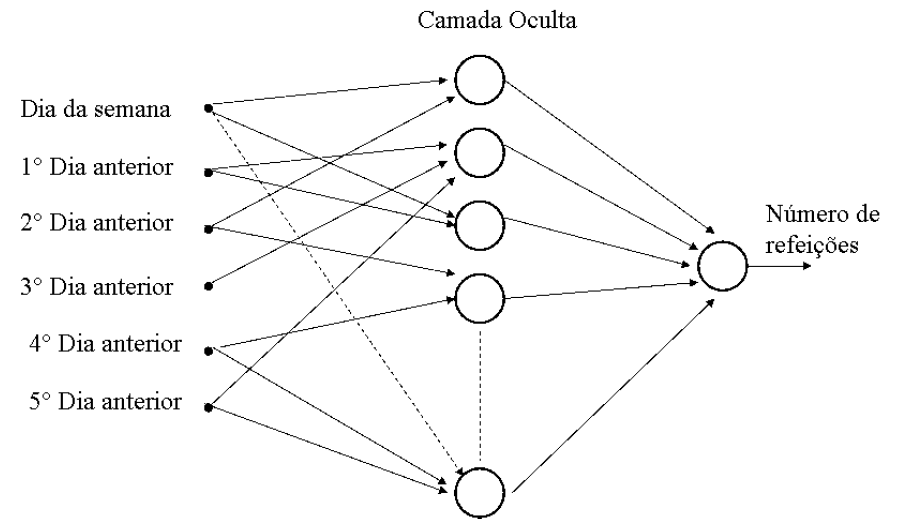
\includegraphics[width=\textwidth]
        {./Figs/15-rna-lopes.png}
        \caption{Rede Neural Perceptron de Múltiplas Camadas.}\caption*{  Fonte:\cite{Lopes2008}.}\label{fig:mlp-lopes}}
        \end{figure}
        
        \citeonline{Rocha2011} também realiza o estudo de demanda no restaurante universitário da Universidade Estadual Paulista Júlio de Mesquita Filho (UNESP), novamente com os métodos de redes neurais artificiais com backpropagation e utilizando apenas como fonte de dados (o histórico numérico das vendas realizadas), e outras variáveis intermediárias obtidas a partir deste, como médias de subconjunto de observações (médias de segundas-feiras). A única variável de ambiente coletada foi o número de feriados próximos à observação de venda. No estudo do total de dias analisados, verifica-se que em 73\% (187 dias), o método de média simples propiciou um maior erro em relação à RNA, que por sua vez ocasionou um erro maior nos 23\% (69 dias) restantes.Em se tratando de menor desperdício, observa-se que a RNA apresenta erros maiores que 50 refeições em 13 dias, enquanto o método da média simples apresenta erros maiores que 50 refeições em 58 dias, concluindo-se então que o método de RNA foi bem mais eficiente do que o cálculo de média simples utilizado pela administração do restaurante universitário. A Figura \ref{fig:rnaRocha} apresenta um esquema da rede  neural aplicada nesse trabalho. 
        \begin{figure}[h]
        \center{
        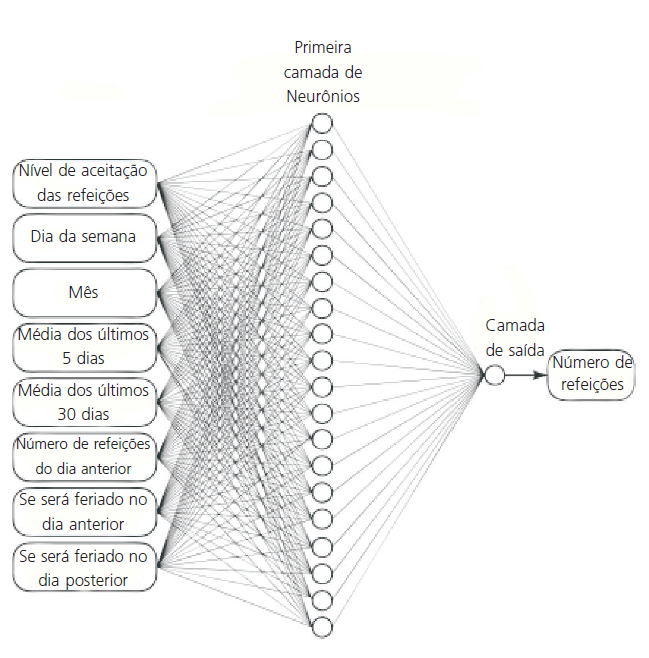
\includegraphics[width=0.8\textwidth]
        {./Figs/16-rna-rocha.png}
        \caption{Rede Neural Perceptron de Múltiplas Camadas}\caption*{ Fonte: \cite{Rocha2011}} \label{fig:rnaRocha}}
        \end{figure}
        
        Tanto o modelo apresentado em \cite{Rocha2011} quando em \cite{Lopes2008} possuem uma única camada oculta. 
      
    \section{Previsão de demanda em outros ambientes}
        \citeonline{RUAS2012} faz uma análise de previsão de demanda de energia elétrica no estado do Paraná, entre os anos de 2004 e 2006, utilizando redes neurais artificiais e máquinas de vetores de suporte. Apesar de não ser o mesmo exemplo do cenário do restaurante universitário do ICT-Unifesp, temos a distribuição dos dados de consumo coletados como uma série temporal. Nesta pesquisa de previsão de demanda de energia elétrica foi utilizada uma rede parcialmente recorrente de Elman, que permite a previsão de um passo de tempo à frente. Para que seja possível realizar a previsão para vários pontos à frente, é necessário utilizar os valores já previstos, ou seja, a saída da rede, como entradas da mesma.
        
        \citeonline{Almeida2013} analisa um cenário semelhante de demanda de energia elétrica, porém utilizando-se técnicas de previsão de demanda com Rede Neural Artificial do tipo Multilayer Perceptron combinado com lógica fuzzy que permite colocar variáveis de temperatura (entre outras) em um conjunto de regras que impactam no problema.
        
        \citeonline{Silva2010} também aplica técnicas de redes neurais para previsão de demanda de energia elétrica, com o estudo de variáveis climáticas, porém através de um modelo de MAPA SOM - (Self-Organizing Map) que é um tipo de rede neural desenvolvido para reconhecimento de padrões. Apesar de ser um modelo não supervisionado, o modelo é ideal para organizar as principais variáveis impactantes e descartáveis na previsão. O mapa som utilizado pelo autor apresenta os dados associados aos seus neurônios de forma que padrões similares encontram-se em neurônios contíguos, tendo uma organização topológica. Deste modo é possível se extrair relações abstratas entre as variáveis do vetor de dados através da sua posição nos mapas componentes, que por meio de uma escala de cores mostram a quantidade de uma variável específica em cada neurônio do mapa.